\documentclass[11pt]{article}
\usepackage[T1]{fontenc}
\usepackage{mathptmx}
\usepackage[margin=1in]{geometry}
\usepackage{longtable,graphicx,amsmath}
\newcommand{\toprule}{\hline}\newcommand{\midrule}{\hline}\newcommand{\bottomrule}{\hline}
\renewcommand{\baselinestretch}{1.12}
\title{Hindcast validation of a structure-weighted mutation early-warning engine on SARS-CoV-2: one early catch, a failed pre-registered bar, and a small unproven precision edge}
\author{B18 validation slice, outbreak-mutation-early-warning}
\date{Closeout of committed results, base commit 51d9d70}
\begin{document}
\maketitle
\begin{abstract}
Mutation early-warning is a crowded area. We validate one reference engine that ranks rising amino-acid mutations by growth rate weighted by structural criticality derived from public antibody--spike and ACE2--spike complexes. Validation used a byte-locked open snapshot (LAPIS v2, 91 weekly bins, 2.84 million sequences) and a gate file committed before any result. The pre-registered catch test \emph{failed}: one of three controls was flagged before literature recognition (bar: two). S:N501Y was flagged 48 days before recognition; S:D614G and S:L452R were never flagged. A growth-only comparator caught exactly the same control at the same freeze. Reaching even this outcome required two methodological pivots after failed runs, both preserved. In a May--August 2021 negative-control window, the weighted rule had precision 0.750 (24/32) against 0.714 (30/42) for growth-only; the difference is not significant (Fisher $p=0.80$). A byproduct finding is that log-proportion slopes are not time-invariant across roughly 100-fold growth in sequencing volume, so no single global slope threshold is valid across eras. We present this as a qualified result, not a win.
\end{abstract}

\section{Introduction}
Genomic surveillance produces thousands of candidate mutations each week. An early-warning engine must flag the few that matter before they are recognized in the literature, without burying analysts in false alarms. The question tested here is narrow: does adding structural criticality to a growth signal help, on a retrospective hindcast with pre-written controls?

We report the validation honestly, including what failed. The protocol was fixed in a gate file (commit 209667f) before any test result existed. When the first run failed, we amended the gates, kept the failure in history, and reran, twice. Section~\ref{sec:pivots} lists each step. The final outcome is a qualified result: one early catch, a failed catch bar, and a point-estimate precision edge that cannot be distinguished from chance.

\paragraph{Contributions.} (i) A frozen-window hindcast with controls chosen in advance. (ii) A complete record of the failures and their root causes. (iii) A measured finding about slope non-stationarity. (iv) A negative-control precision comparison with an explicit significance test. We do not claim the engine outperforms growth-only ranking.

\section{Related work}
The area is crowded. \textbf{VirusWarn} (doi:10.1016/j.csbj.2025.03.010) flags variants by mutation burden and rule lists against known variants of concern; it is composition-based and retrospective. \textbf{FEVER} (doi:10.1371/journal.pgph.0000207) couples biosurveillance with mutation typing and estimates empirical risk from lineage outcomes; it is statistical and has no structural model. \textbf{CoVerage} (doi:10.1038/s41467-025-60231-4) scores spike mutations antigenically alongside epidemiological dynamics and is the closest in aim; its score is a curated literature score. \textbf{Nextstrain} (doi:10.1093/bioinformatics/bty400) provides real-time phylogenetic tracking and visualization and does not rank mutations by predicted impact. These were checked on 2026-09-23 as recorded in the gate file; they were not re-checked at closeout. Our stated angle was criticality derived from PDB contact geometry. Our results do not show that this angle improves on growth alone.

\section{Data}
Counts come from the LAPIS open v2 instance (dataset sars\_cov-2\_nextstrain\_open), snapshot dataVersion 1790179197, fetched 2026-09-23. Weekly amino-acid mutation tables use a minimum proportion of 0.001; daily sequence totals cover 2019-12-30 to 2021-10-04. The raw JSON is byte-locked (commit bfa76d8, MANIFEST\_DATA\_CODE.sha256). Structural data are PDB 6M0J (ACE2--RBD), 6WPT, 6XDG and 7C2L (antibody--spike complexes), with SARS-CoV-2 and SARS-CoV-1 spike references.

A measurement fix applies to the final run. Counts from the mutation endpoint and totals from the daily endpoint use different date fields, so count divided by total can exceed 1. Shares used in truth labelling and trajectories therefore use the LAPIS \texttt{proportion} field.

\section{Method}
\subsection{Candidates and growth}
At a freeze date $F$, only weeks ending on or before $F$ are used. A mutation is a candidate if its count in the last four weeks is at least 20, its four-week proportion is at least 0.001, and its growth slope $g$ is positive. $g$ is the slope of $\log_{10}\big((c+0.5)/(n+1)\big)$ over the last six visible weeks, where $c$ is count and $n$ is the weekly total. After the first pivot, the fit uses observed weeks only and requires at least four of six.

\subsection{Structural score}
For spike mutations,
\begin{equation}
S = 0.35\,E + 0.25\,I + 0.15\,C + 0.15\,D + 0.10\,K,
\end{equation}
where $E$ marks residues within 5~\AA\ of a partner chain in 6WPT, 6XDG or 7C2L, $I$ marks the ACE2 interface in 6M0J, $C$ marks cleavage sites (681--685, 815), $D$ marks critical domains (RBM 437--508, fusion peptide 816--837, HR1 920--970), and $K$ marks conservation against SARS-CoV-1. Non-spike mutations have $S=0$; this is a real limitation. The alert score is $A=g\,(0.5+S)$.

\subsection{Detection rules}
\emph{Locked rule.} Flag if $g\ge G_{\min}$ and $A\ge\Theta$. \emph{Final rule} (second amendment). Within each scan, compute the robust $z$-score $z_A=(A-\mathrm{med}(A))/(1.4826\,\mathrm{MAD}(A))$ over the candidate set and flag if $z_A\ge Z$ with $Z=6.6$. The growth-only comparator applies the same per-scan $z$ to $g$ with $Z_G=4.8$. Both constants come from one calibration budget rule on four disjoint freezes (2020-05-31 to 2020-08-31): at most three alerts per scan for the weighted rule, and at most 12 total for growth-only.

\subsection{Protocol}
Monthly freezes run from 2020-01-31 to 2021-09-30. The positive controls and recognition dates were fixed beforehand: S:D614G (2020-04-30; Korber et al., doi:10.1101/2020.04.29.069054), S:N501Y (2020-12-18; COG-UK preliminary characterisation), S:L452R (2021-01-17; CDPH release NR21-020). The pass bar is at least two of three flagged at a freeze strictly before recognition. For the negative-control window (freezes 2021-05-31 through 2021-08-31), alerts are deduplicated at first flag, and an alert is a true positive if the mutation reaches 20\% of weekly sequences within 26 weeks. Precision is true positives over all alerts.

\section{The pivot chain}\label{sec:pivots}
Table~\ref{tab:pivots} lists the runs. All five commits are in the repository history.
\begin{table}[h]\centering\small
\begin{tabular}{llp{6.2cm}}\toprule
Step & Commit & Outcome\\\midrule
Locked gates & 209667f & Committed before any result\\
Locked run & 55bd7e1 & 0/3 controls; negative window: 4 weighted alerts, 150 growth-only alerts, 0 true positives\\
Amendment 1 & 47f1a7f & Observed-weeks slope; constants re-derived\\
Amendment 1 run & 04d9280 & 0/3 controls; 0 alerts in negative window\\
Amendment 2 & b08e624 & Per-scan robust $z$; $Z=6.6$, $Z_G=4.8$\\
Final run & 51d9d70 & 1/3 controls; precision 0.750 vs 0.714\\\bottomrule
\end{tabular}\caption{Pivot chain. Each amendment was committed before its own rerun.}\label{tab:pivots}
\end{table}

\subsection{Root cause 1: censored weeks fit as zeros}
The 6-week slope treated weeks below the 0.1\% query floor as zero counts, which anchors the log value near $-7$. In the calibration window, noise mutations that cross the floor receive huge slopes, so the 95th-percentile threshold $G_{\min}=0.4141$ measured floor artifacts. Genuine risers observed in all six weeks had modest slopes (N501Y about 0.2 per week) and fell below it. Below-floor weeks are censored, not zero.

\subsection{Root cause 2: slopes are not time-invariant}
With the estimator fixed, calibration on May--August 2020 gave $G_{\min}=0.2347$. That is above the true slope of the defining Delta RBD mutation S:T478K (0.224 at 2021-05-31). Sequencing volume grew about 100-fold over the study period, which compresses log-proportion slopes in later eras. No single global slope threshold separates signal from noise across eras. This is a finding about the signal, not only about our engine, and it motivates per-scan normalisation.

\subsection{What the pivots cost}
The second amendment's diagnosis used a slope measured inside the negative-control window, and the first amendment described itself as the single pivot. The final rule is therefore not a clean pre-registered test. We changed the method between runs twice and report the result of the last of three runs. Readers should treat the final numbers as exploratory.

\section{Results}
\subsection{Catch test}
Table~\ref{tab:catch} and Figure~\ref{fig:controls} give the controls. One of three was caught, so the pre-registered bar of two was \textbf{not met}. We did not retune after seeing this.
\begin{table}[h]\centering\small
\begin{tabular}{lllll}\toprule
Control & Recognition & First flag (weighted) & Lead (days) & Growth-only\\\midrule
S:D614G & 2020-04-30 & never & -- & never\\
S:N501Y & 2020-12-18 & 2020-10-31 & 48 & 2020-10-31\\
S:L452R & 2021-01-17 & never & -- & never\\\bottomrule
\end{tabular}\caption{Catch test under the final rule. Both rules pass 1 of 3; the bar is 2 of 3.}\label{tab:catch}
\end{table}
\begin{figure}[h]\centering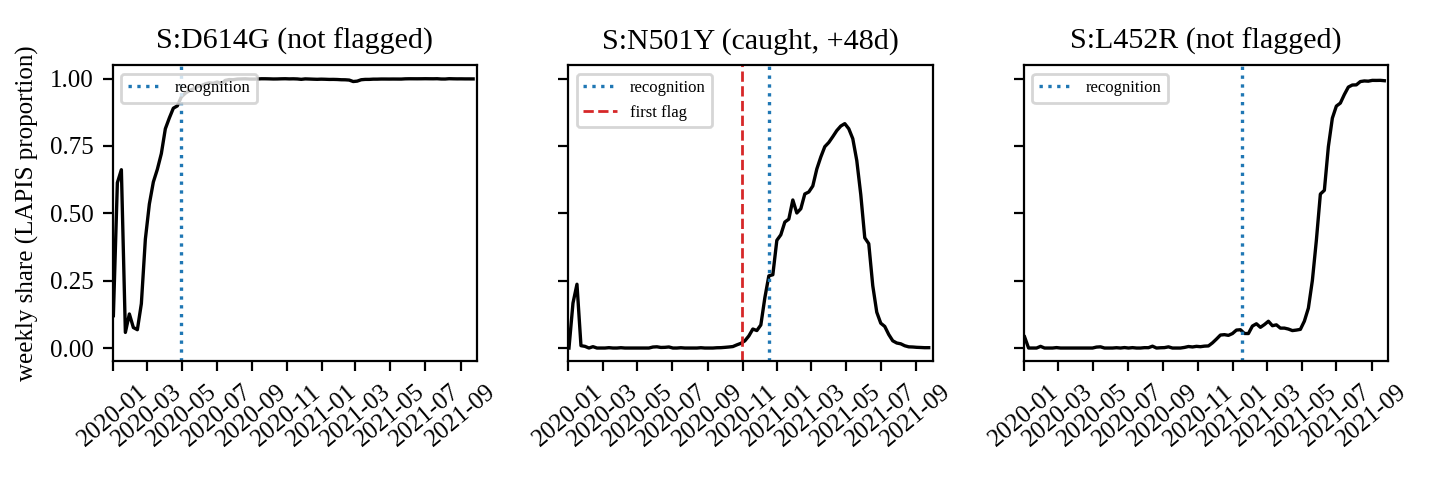
\includegraphics[width=\textwidth]{../figures/fig1_control_trajectories.png}
\caption{Weekly share of the three controls. Dotted: recognition date. Dashed: first flag (N501Y only).}\label{fig:controls}\end{figure}

\paragraph{Why the negatives.} D614G was already near 90\% share by the first scan with usable data, so almost none of its rise fell inside the scan schedule; this control was a poor choice for a monthly-freeze design, and we cannot say the engine would have missed it under finer cadence. L452R sat on a long low plateau (roughly 5--10\% share from November 2020 to March 2021) before rising, so its growth signal was weak until after recognition. N501Y was flagged at about 2\% share. Three controls cannot support a rate estimate.

\subsection{Growth-only comparison on the catch test}
The comparator flagged N501Y at the same freeze, for the same 48 days of lead. Structural weighting added no catch advantage on these controls.

\subsection{Negative-control precision}
\begin{figure}[h]\centering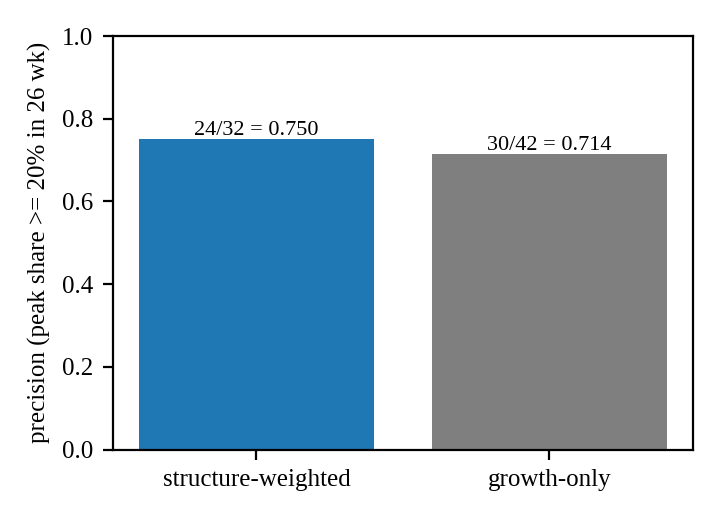
\includegraphics[width=0.55\textwidth]{../figures/fig3_precision.png}
\caption{Precision in the May--August 2021 window.}\label{fig:prec}\end{figure}
The weighted rule issued 32 alerts (24 true positives, 0.750). Growth-only issued 42 (30 true positives, 0.714). Thirty-one alerts are shared; the weighted rule has one that growth-only lacks (S:T250I) and growth-only has 11 the weighted rule lacks, all non-spike. Only 7 of 32 weighted alerts have $S>0$. The weighted rule is therefore close to a thinned growth-only list. A two-sided Fisher exact test on the two $2\times2$ tables gives $p=0.796$. The pre-stated claim that structural weighting improves precision is not supported at any usable confidence. The point difference is 0.036.

The weighted rule flagged the full Delta constellation (S:T478K, S:P681R, S:G142D, S:D950N) at the 2021-05-31 freeze (Figure~\ref{fig:delta}), when these mutations were near 50\% share. This is a detection of a variant already spreading fast, not an early warning.
\begin{figure}[h]\centering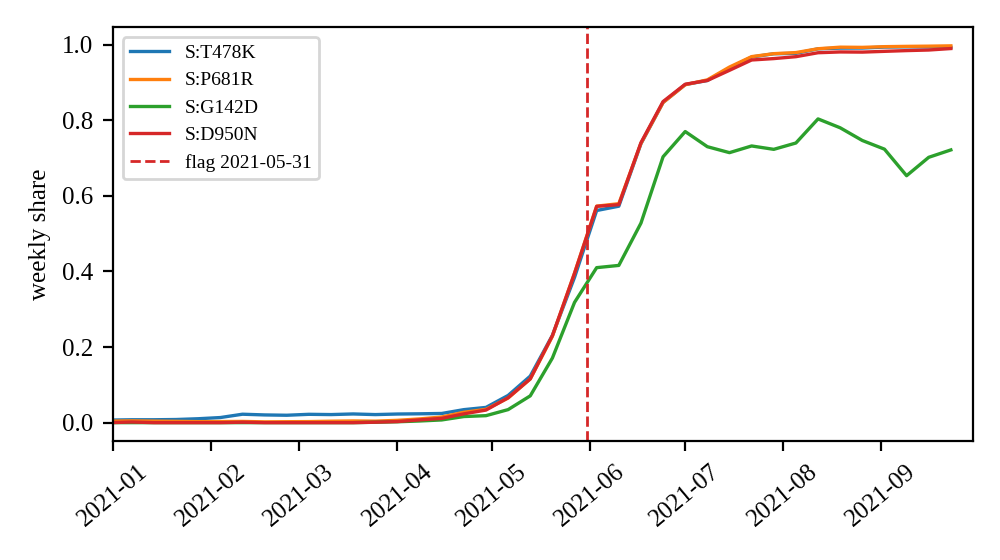
\includegraphics[width=0.75\textwidth]{../figures/fig2_delta_constellation.png}
\caption{Delta constellation trajectories; dashed line is the flag date.}\label{fig:delta}\end{figure}

\subsection{Alert load}
\begin{figure}[h]\centering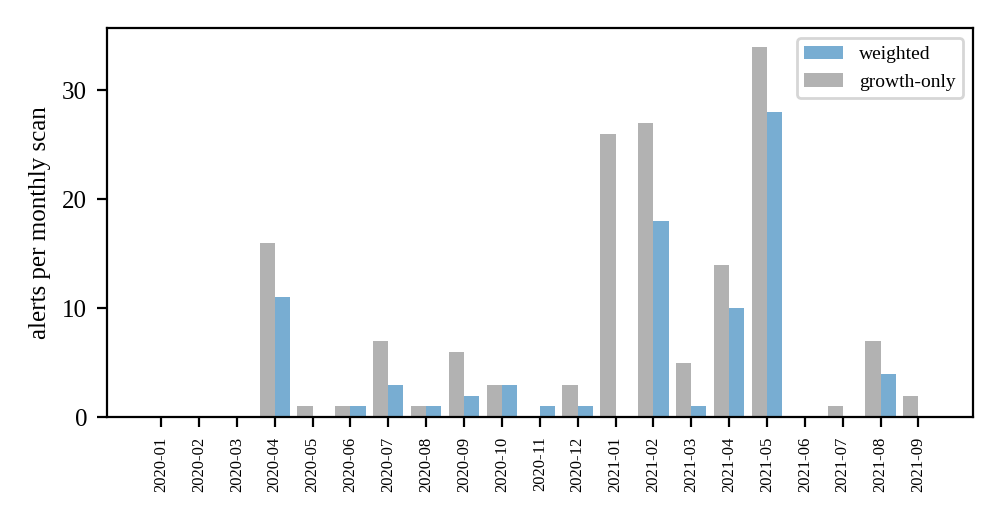
\includegraphics[width=0.85\textwidth]{../figures/fig4_alerts_per_scan.png}
\caption{Alerts per monthly scan under both rules.}\label{fig:load}\end{figure}
Figure~\ref{fig:load} shows that alert load is bursty: the busiest scans (2021-01, 2021-02, 2021-05) coincide with variant sweeps and carry many linked hitchhiker mutations. Appendix~\ref{app:scan} lists the counts.

\section{Discussion}
\paragraph{What the evidence supports.} The engine, run on frozen data, flagged one documented concerning mutation 48 days before recognition. Nothing else in the catch test supports an early-warning claim. The reproduction of the committed results from byte-locked inputs was confirmed independently (the regenerated results file is byte-identical), so the numbers are reliable even though their interpretation is limited.

\paragraph{What it does not support.} It does not show that structural criticality improves ranking. With $S=0$ outside spike, and most alerts outside spike, the structural term touches few candidates. It does not show the engine generalises beyond this virus and snapshot. It does not establish a catch rate.

\paragraph{Truth definition.} Labelling an alert correct if the mutation reaches 20\% share rewards flagging hitchhikers on a sweeping lineage. Precision values mix independent detections with linked mutations, and an evaluation that clusters alerts by lineage would be more informative.

\paragraph{The slope result.} The most reusable finding is that a fixed growth threshold calibrated in one sequencing era fails in another. Any operational scanner using log-proportion slope needs era or volume normalisation, as the per-scan $z$-score provides, at the cost of making alert counts depend on each scan's own candidate set.

\section{Threats to validity}
\begin{enumerate}
\item \textbf{Forking paths.} Three rule versions (locked plus two amendments) were run on the same test windows; later versions were informed by earlier failures, including a slope from the negative window.
\item \textbf{Three controls.} Coarse by design; one control decides the bar.
\item \textbf{Control cadence.} Monthly freezes cannot resolve a mutation already dominant at the first usable scan.
\item \textbf{Spike-only structure.} The weighted score is zero for most genome positions.
\item \textbf{Retrospective snapshot.} A snapshot fetched after the fact omits submission delay and later reclassification.
\item \textbf{Truth definition.} Twenty percent share within 26 weeks is ad hoc and confounded by linkage.
\item \textbf{Prior art.} Related-work checks date from 2026-09-23.
\end{enumerate}

\section{Conclusion}
The reference engine produced one early catch (N501Y, 48 days), failed its pre-registered catch bar, and showed a precision difference over growth-only ranking that is within noise. The pivots that produced even this result are documented and reproducible. The engine is a usable scanner with a validated detection rule, not a demonstrated improvement over growth-only ranking. A follow-up needs more controls chosen in advance, finer scan cadence, lineage-clustered truth labels, and a test window untouched by method development.

\section*{Reproducibility}
Code: \texttt{validation/code/run\_validation.py} (engine in \texttt{engine\_fast.py}); figures and derived statistics: \texttt{make\_figures.py}. Inputs are byte-locked under \texttt{validation/data}. Hashes: \texttt{validation/MANIFEST.sha256}. The gate files and pivot commits are the audit trail.

\appendix
\section{Monthly scan alert counts}\label{app:scan}
{\small\begin{longtable}{lrr}
\toprule Freeze & Weighted alerts & Growth-only alerts\\\midrule
\endhead
2020-01-31 & 0 & 0\\
2020-02-29 & 0 & 0\\
2020-03-31 & 0 & 0\\
2020-04-30 & 11 & 16\\
2020-05-31 & 0 & 1\\
2020-06-30 & 1 & 1\\
2020-07-31 & 3 & 7\\
2020-08-31 & 1 & 1\\
2020-09-30 & 2 & 6\\
2020-10-31 & 3 & 3\\
2020-11-30 & 1 & 0\\
2020-12-31 & 1 & 3\\
2021-01-31 & 0 & 26\\
2021-02-28 & 18 & 27\\
2021-03-31 & 1 & 5\\
2021-04-30 & 10 & 14\\
2021-05-31 & 28 & 34\\
2021-06-30 & 0 & 0\\
2021-07-31 & 0 & 1\\
2021-08-31 & 4 & 7\\
2021-09-30 & 0 & 2\\
\bottomrule
\end{longtable}}
\section{Negative-control alerts, structure-weighted rule}
{\footnotesize\begin{longtable}{lrrrrrc}
\toprule Mutation & Flag & $g$ & $S$ & $A$ & Peak 26wk & TP\\\midrule
\endhead
S:T478K & 2021-05-31 & 0.224 & 0.50 & 0.224 & 0.994 & yes\\
S:W152R & 2021-05-31 & 0.254 & 0.35 & 0.216 & 0.043 & no\\
ORF1a:A2529V & 2021-05-31 & 0.401 & 0.00 & 0.200 & 0.502 & yes\\
S:D950N & 2021-05-31 & 0.261 & 0.25 & 0.196 & 0.990 & yes\\
ORF1a:V2930L & 2021-05-31 & 0.328 & 0.00 & 0.164 & 0.936 & yes\\
ORF1a:A1306S & 2021-05-31 & 0.327 & 0.00 & 0.164 & 0.937 & yes\\
N:G215C & 2021-05-31 & 0.327 & 0.00 & 0.163 & 0.930 & yes\\
ORF1b:A1918V & 2021-05-31 & 0.326 & 0.00 & 0.163 & 0.937 & yes\\
S:P681R & 2021-05-31 & 0.247 & 0.15 & 0.161 & 0.997 & yes\\
ORF7b:T40I & 2021-05-31 & 0.316 & 0.00 & 0.158 & 0.935 & yes\\
ORF1a:T3646A & 2021-05-31 & 0.300 & 0.00 & 0.150 & 0.937 & yes\\
ORF1a:P2046L & 2021-05-31 & 0.297 & 0.00 & 0.148 & 0.936 & yes\\
ORF1a:P2287S & 2021-05-31 & 0.289 & 0.00 & 0.145 & 0.926 & yes\\
ORF1a:S2048F & 2021-05-31 & 0.276 & 0.00 & 0.138 & 0.020 & no\\
S:R158G & 2021-05-31 & 0.273 & 0.00 & 0.137 & 0.988 & yes\\
ORF8:D119- & 2021-05-31 & 0.273 & 0.00 & 0.137 & 0.991 & yes\\
ORF8:F120- & 2021-05-31 & 0.273 & 0.00 & 0.137 & 0.989 & yes\\
S:F157- & 2021-05-31 & 0.273 & 0.00 & 0.136 & 0.989 & yes\\
S:G142D & 2021-05-31 & 0.273 & 0.00 & 0.136 & 0.803 & yes\\
S:E156- & 2021-05-31 & 0.273 & 0.00 & 0.136 & 0.987 & yes\\
ORF9b:T60A & 2021-05-31 & 0.269 & 0.00 & 0.134 & 0.992 & yes\\
N:D63G & 2021-05-31 & 0.269 & 0.00 & 0.134 & 0.988 & yes\\
S:T19R & 2021-05-31 & 0.268 & 0.00 & 0.134 & 0.993 & yes\\
S:G1124V & 2021-05-31 & 0.223 & 0.10 & 0.134 & 0.008 & no\\
ORF1a:K4224R & 2021-05-31 & 0.266 & 0.00 & 0.133 & 0.006 & no\\
ORF7a:T120I & 2021-05-31 & 0.263 & 0.00 & 0.132 & 0.985 & yes\\
ORF1b:G662S & 2021-05-31 & 0.262 & 0.00 & 0.131 & 0.996 & yes\\
ORF1b:P1000L & 2021-05-31 & 0.257 & 0.00 & 0.129 & 0.995 & yes\\
ORF1a:A2355S & 2021-08-31 & 0.437 & 0.00 & 0.218 & 0.037 & no\\
ORF1b:P2313S & 2021-08-31 & 0.249 & 0.00 & 0.125 & 0.005 & no\\
S:T250I & 2021-08-31 & 0.125 & 0.35 & 0.106 & 0.008 & no\\
S:I850L & 2021-08-31 & 0.170 & 0.10 & 0.102 & 0.013 & no\\
\bottomrule
\end{longtable}}
\section{Negative-control alerts, growth-only comparator}
{\footnotesize\begin{longtable}{lrrrrrc}
\toprule Mutation & Flag & $g$ & $S$ & $A$ & Peak 26wk & TP\\\midrule
\endhead
S:T478K & 2021-05-31 & 0.224 & 0.50 & 0.224 & 0.994 & yes\\
S:W152R & 2021-05-31 & 0.254 & 0.35 & 0.216 & 0.043 & no\\
ORF1a:A2529V & 2021-05-31 & 0.401 & 0.00 & 0.200 & 0.502 & yes\\
S:D950N & 2021-05-31 & 0.261 & 0.25 & 0.196 & 0.990 & yes\\
ORF1a:V2930L & 2021-05-31 & 0.328 & 0.00 & 0.164 & 0.936 & yes\\
ORF1a:A1306S & 2021-05-31 & 0.327 & 0.00 & 0.164 & 0.937 & yes\\
N:G215C & 2021-05-31 & 0.327 & 0.00 & 0.163 & 0.930 & yes\\
ORF1b:A1918V & 2021-05-31 & 0.326 & 0.00 & 0.163 & 0.937 & yes\\
S:P681R & 2021-05-31 & 0.247 & 0.15 & 0.161 & 0.997 & yes\\
ORF7b:T40I & 2021-05-31 & 0.316 & 0.00 & 0.158 & 0.935 & yes\\
ORF1a:T3646A & 2021-05-31 & 0.300 & 0.00 & 0.150 & 0.937 & yes\\
ORF1a:P2046L & 2021-05-31 & 0.297 & 0.00 & 0.148 & 0.936 & yes\\
ORF1a:P2287S & 2021-05-31 & 0.289 & 0.00 & 0.145 & 0.926 & yes\\
ORF1a:S2048F & 2021-05-31 & 0.276 & 0.00 & 0.138 & 0.020 & no\\
S:R158G & 2021-05-31 & 0.273 & 0.00 & 0.137 & 0.988 & yes\\
ORF8:D119- & 2021-05-31 & 0.273 & 0.00 & 0.137 & 0.991 & yes\\
ORF8:F120- & 2021-05-31 & 0.273 & 0.00 & 0.137 & 0.989 & yes\\
S:F157- & 2021-05-31 & 0.273 & 0.00 & 0.136 & 0.989 & yes\\
S:G142D & 2021-05-31 & 0.273 & 0.00 & 0.136 & 0.803 & yes\\
S:E156- & 2021-05-31 & 0.273 & 0.00 & 0.136 & 0.987 & yes\\
ORF9b:T60A & 2021-05-31 & 0.269 & 0.00 & 0.134 & 0.992 & yes\\
N:D63G & 2021-05-31 & 0.269 & 0.00 & 0.134 & 0.988 & yes\\
S:T19R & 2021-05-31 & 0.268 & 0.00 & 0.134 & 0.993 & yes\\
S:G1124V & 2021-05-31 & 0.223 & 0.10 & 0.134 & 0.008 & no\\
ORF1a:K4224R & 2021-05-31 & 0.266 & 0.00 & 0.133 & 0.006 & no\\
ORF7a:T120I & 2021-05-31 & 0.263 & 0.00 & 0.132 & 0.985 & yes\\
ORF1b:G662S & 2021-05-31 & 0.262 & 0.00 & 0.131 & 0.996 & yes\\
ORF1b:P1000L & 2021-05-31 & 0.257 & 0.00 & 0.129 & 0.995 & yes\\
N:R203M & 2021-05-31 & 0.255 & 0.00 & 0.127 & 0.991 & yes\\
ORF7a:V82A & 2021-05-31 & 0.255 & 0.00 & 0.127 & 0.986 & yes\\
ORF3a:S26L & 2021-05-31 & 0.248 & 0.00 & 0.124 & 0.997 & yes\\
N:D377Y & 2021-05-31 & 0.237 & 0.00 & 0.118 & 0.987 & yes\\
ORF1a:T3255I & 2021-05-31 & 0.225 & 0.00 & 0.113 & 0.937 & yes\\
M:I82T & 2021-05-31 & 0.210 & 0.00 & 0.105 & 0.998 & yes\\
N:A208S & 2021-07-31 & 0.330 & 0.00 & 0.165 & 0.018 & no\\
ORF1a:A2355S & 2021-08-31 & 0.437 & 0.00 & 0.218 & 0.037 & no\\
ORF1b:P2313S & 2021-08-31 & 0.249 & 0.00 & 0.125 & 0.005 & no\\
S:I850L & 2021-08-31 & 0.170 & 0.10 & 0.102 & 0.013 & no\\
ORF3a:K16T & 2021-08-31 & 0.175 & 0.00 & 0.087 & 0.013 & no\\
ORF8:I88T & 2021-08-31 & 0.159 & 0.00 & 0.079 & 0.007 & no\\
ORF1b:D2576G & 2021-08-31 & 0.154 & 0.00 & 0.077 & 0.008 & no\\
N:S232G & 2021-08-31 & 0.154 & 0.00 & 0.077 & 0.004 & no\\
\bottomrule
\end{longtable}}
\section{Constants by rule version}
\begin{table}[h]\centering\small
\begin{tabular}{lll}\toprule
Version & Constants & Calibration set\\\midrule
Locked & $G_{\min}=0.4141$, $\Theta=0.4716$, $\Theta_G=0.6088$ & 1923 candidates\\
Amendment 1 & $G_{\min}=0.2347$, $\Theta=0.3525$, $\Theta_G=0.4663$ & 960 candidates\\
Amendment 2 (final) & $Z=6.6$, $Z_G=4.8$ & same four freezes\\\bottomrule
\end{tabular}\end{table}
\end{document}
